\documentclass[11pt]{article}
\usepackage{physics}
% NOTE: Add in the relevant information to the commands below; or, if you'll be using the same information frequently, add these commands at the top of paolo-pset.tex file. 
\newcommand{\name}{TA: Hossein Mohammadi}
\newcommand{\email}{hossein.mohammadi.00427@gmail.com}
\newcommand{\classnum}{Advanced Quantum Field Theory}
\newcommand{\subject}{Subject: Casimir Energy and point particle quantization}
\newcommand{\instructors}{Dr. Amin Faraji}
\newcommand{\assignment}{PSet 3}
\newcommand{\semester}{- Fall 1402}
\newcommand{\duedate}{dd/mm/yyyy}

% Copyright 2021 Paolo Adajar (padajar.com, paoloadajar@mit.edu)
% 
% Permission is hereby granted, free of charge, to any person obtaining a copy of this software and associated documentation files (the "Software"), to deal in the Software without restriction, including without limitation the rights to use, copy, modify, merge, publish, distribute, sublicense, and/or sell copies of the Software, and to permit persons to whom the Software is furnished to do so, subject to the following conditions:
%
% The above copyright notice and this permission notice shall be included in all copies or substantial portions of the Software.
% 
% THE SOFTWARE IS PROVIDED "AS IS", WITHOUT WARRANTY OF ANY KIND, EXPRESS OR IMPLIED, INCLUDING BUT NOT LIMITED TO THE WARRANTIES OF MERCHANTABILITY, FITNESS FOR A PARTICULAR PURPOSE AND NONINFRINGEMENT. IN NO EVENT SHALL THE AUTHORS OR COPYRIGHT HOLDERS BE LIABLE FOR ANY CLAIM, DAMAGES OR OTHER LIABILITY, WHETHER IN AN ACTION OF CONTRACT, TORT OR OTHERWISE, ARISING FROM, OUT OF OR IN CONNECTION WITH THE SOFTWARE OR THE USE OR OTHER DEALINGS IN THE SOFTWARE.

\usepackage{fullpage}
\usepackage{enumitem}
\usepackage{amsfonts, amssymb, amsmath,amsthm}
\usepackage{mathtools}
\usepackage[pdftex, pdfauthor={\name}, pdftitle={\classnum~\assignment}]{hyperref}
\usepackage[dvipsnames]{xcolor}
\usepackage{bbm}
\usepackage{graphicx}
\usepackage{mathrsfs}
\usepackage{pdfpages}
\usepackage{tabularx}
\usepackage{pdflscape}
\usepackage{makecell}
\usepackage{booktabs}
\usepackage{natbib}
\usepackage{caption}
\usepackage{subcaption}
\usepackage{physics}
\usepackage[many]{tcolorbox}
\usepackage{version}
\usepackage{ifthen}
\usepackage{cancel}
\usepackage{listings}
\usepackage{courier}

\usepackage{tikz}
\usepackage{istgame}
\usepackage{Float}

\hypersetup{
	colorlinks=true,
	linkcolor=blue,
	filecolor=magenta,
	urlcolor=blue,
}

\setlength{\parindent}{0mm}
\setlength{\parskip}{2mm}

\setlist[enumerate]{label=({\alph*})}
\setlist[enumerate, 2]{label=({\roman*})}

\allowdisplaybreaks[1]

\newcommand{\psetheader}{
	\ifthenelse{\isundefined{\collaborators}}{
		\begin{center}
			{\setlength{\parindent}{0cm} \setlength{\parskip}{0mm}
				
				\textbf{\classnum~\semester:~\assignment} \hfill \name
				
				
				\subject \hfill %\href{mailto:\email}{\tt \email}
				
				Instructor:~\instructors \hfill Due Date:~\duedate	
				
				\hrulefill}
		\end{center}
	}{
		\begin{center}
			{\setlength{\parindent}{0cm} \setlength{\parskip}{0mm}
				
				{\textbf{\classnum~\semester:~\assignment} \hfill \name\footnote{Collaborator(s): \collaborators}}
				
				\subject \hfill \href{mailto:\email}{\tt \email}
				
				Instructor(s):~\instructors \hfill Due Date:~\duedate	
				
				\hrulefill}
		\end{center}
	}
}

\renewcommand{\thepage}{\classnum~\assignment \hfill \arabic{page}}

\makeatletter
\def\points{\@ifnextchar[{\@with}{\@without}}
\def\@with[#1]#2{{\ifthenelse{\equal{#2}{1}}{{[1 point, #1]}}{{[#2 points, #1]}}}}
\def\@without#1{\ifthenelse{\equal{#1}{1}}{{[1 point]}}{{[#1 points]}}}
\makeatother

\newtheoremstyle{theorem-custom}%
{}{}%
{}{}%
{\itshape}{.}%
{ }%
{\thmname{#1}\thmnumber{ #2}\thmnote{ (#3)}}

\theoremstyle{theorem-custom}

\newtheorem{theorem}{Theorem}
\newtheorem{lemma}[theorem]{Lemma}
\newtheorem{example}[theorem]{Example}

\newenvironment{problem}[1]{\color{black} #1}{}

\newenvironment{solution}{%
	\leavevmode\begin{tcolorbox}[breakable, colback=green!5!white,colframe=green!75!black, enhanced jigsaw] \proof[\scshape Solution:] \setlength{\parskip}{2mm}%
	}{\renewcommand{\qedsymbol}{$\blacksquare$} \endproof \end{tcolorbox}}

\newenvironment{reflection}{\begin{tcolorbox}[breakable, colback=black!8!white,colframe=black!60!white, enhanced jigsaw, parbox = false]\textsc{Reflections:}}{\end{tcolorbox}}

\newcommand{\qedh}{\renewcommand{\qedsymbol}{$\blacksquare$}\qedhere}

\definecolor{mygreen}{rgb}{0,0.6,0}
\definecolor{mygray}{rgb}{0.5,0.5,0.5}
\definecolor{mymauve}{rgb}{0.58,0,0.82}

% from https://github.com/satejsoman/stata-lstlisting
% language definition
\lstdefinelanguage{Stata}{
	% System commands
	morekeywords=[1]{regress, reg, summarize, sum, display, di, generate, gen, bysort, use, import, delimited, predict, quietly, probit, margins, test},
	% Reserved words
	morekeywords=[2]{aggregate, array, boolean, break, byte, case, catch, class, colvector, complex, const, continue, default, delegate, delete, do, double, else, eltypedef, end, enum, explicit, export, external, float, for, friend, function, global, goto, if, inline, int, local, long, mata, matrix, namespace, new, numeric, NULL, operator, orgtypedef, pointer, polymorphic, pragma, private, protected, public, quad, real, return, rowvector, scalar, short, signed, static, strL, string, struct, super, switch, template, this, throw, transmorphic, try, typedef, typename, union, unsigned, using, vector, version, virtual, void, volatile, while,},
	% Keywords
	morekeywords=[3]{forvalues, foreach, set},
	% Date and time functions
	morekeywords=[4]{bofd, Cdhms, Chms, Clock, clock, Cmdyhms, Cofc, cofC, Cofd, cofd, daily, date, day, dhms, dofb, dofC, dofc, dofh, dofm, dofq, dofw, dofy, dow, doy, halfyear, halfyearly, hh, hhC, hms, hofd, hours, mdy, mdyhms, minutes, mm, mmC, mofd, month, monthly, msofhours, msofminutes, msofseconds, qofd, quarter, quarterly, seconds, ss, ssC, tC, tc, td, th, tm, tq, tw, week, weekly, wofd, year, yearly, yh, ym, yofd, yq, yw,},
	% Mathematical functions
	morekeywords=[5]{abs, ceil, cloglog, comb, digamma, exp, expm1, floor, int, invcloglog, invlogit, ln, ln1m, ln, ln1p, ln, lnfactorial, lngamma, log, log10, log1m, log1p, logit, max, min, mod, reldif, round, sign, sqrt, sum, trigamma, trunc,},
	% Matrix functions
	morekeywords=[6]{cholesky, coleqnumb, colnfreeparms, colnumb, colsof, corr, det, diag, diag0cnt, el, get, hadamard, I, inv, invsym, issymmetric, J, matmissing, matuniform, mreldif, nullmat, roweqnumb, rownfreeparms, rownumb, rowsof, sweep, trace, vec, vecdiag, },
	% Programming functions
	morekeywords=[7]{autocode, byteorder, c, _caller, chop, abs, clip, cond, e, fileexists, fileread, filereaderror, filewrite, float, fmtwidth, has_eprop, inlist, inrange, irecode, matrix, maxbyte, maxdouble, maxfloat, maxint, maxlong, mi, minbyte, mindouble, minfloat, minint, minlong, missing, r, recode, replay, return, s, scalar, smallestdouble,},
	% Random-number functions
	morekeywords=[8]{rbeta, rbinomial, rcauchy, rchi2, rexponential, rgamma, rhypergeometric, rigaussian, rlaplace, rlogistic, rnbinomial, rnormal, rpoisson, rt, runiform, runiformint, rweibull, rweibullph,},
	% Selecting time-span functions
	morekeywords=[9]{tin, twithin,},
	% Statistical functions
	morekeywords=[10]{betaden, binomial, binomialp, binomialtail, binormal, cauchy, cauchyden, cauchytail, chi2, chi2den, chi2tail, dgammapda, dgammapdada, dgammapdadx, dgammapdx, dgammapdxdx, dunnettprob, exponential, exponentialden, exponentialtail, F, Fden, Ftail, gammaden, gammap, gammaptail, hypergeometric, hypergeometricp, ibeta, ibetatail, igaussian, igaussianden, igaussiantail, invbinomial, invbinomialtail, invcauchy, invcauchytail, invchi2, invchi2tail, invdunnettprob, invexponential, invexponentialtail, invF, invFtail, invgammap, invgammaptail, invibeta, invibetatail, invigaussian, invigaussiantail, invlaplace, invlaplacetail, invlogistic, invlogistictail, invnbinomial, invnbinomialtail, invnchi2, invnF, invnFtail, invnibeta, invnormal, invnt, invnttail, invpoisson, invpoissontail, invt, invttail, invtukeyprob, invweibull, invweibullph, invweibullphtail, invweibulltail, laplace, laplaceden, laplacetail, lncauchyden, lnigammaden, lnigaussianden, lniwishartden, lnlaplaceden, lnmvnormalden, lnnormal, lnnormalden, lnwishartden, logistic, logisticden, logistictail, nbetaden, nbinomial, nbinomialp, nbinomialtail, nchi2, nchi2den, nchi2tail, nF, nFden, nFtail, nibeta, normal, normalden, npnchi2, npnF, npnt, nt, ntden, nttail, poisson, poissonp, poissontail, t, tden, ttail, tukeyprob, weibull, weibullden, weibullph, weibullphden, weibullphtail, weibulltail,},
	% String functions 
	morekeywords=[11]{abbrev, char, collatorlocale, collatorversion, indexnot, plural, plural, real, regexm, regexr, regexs, soundex, soundex_nara, strcat, strdup, string, strofreal, string, strofreal, stritrim, strlen, strlower, strltrim, strmatch, strofreal, strofreal, strpos, strproper, strreverse, strrpos, strrtrim, strtoname, strtrim, strupper, subinstr, subinword, substr, tobytes, uchar, udstrlen, udsubstr, uisdigit, uisletter, ustrcompare, ustrcompareex, ustrfix, ustrfrom, ustrinvalidcnt, ustrleft, ustrlen, ustrlower, ustrltrim, ustrnormalize, ustrpos, ustrregexm, ustrregexra, ustrregexrf, ustrregexs, ustrreverse, ustrright, ustrrpos, ustrrtrim, ustrsortkey, ustrsortkeyex, ustrtitle, ustrto, ustrtohex, ustrtoname, ustrtrim, ustrunescape, ustrupper, ustrword, ustrwordcount, usubinstr, usubstr, word, wordbreaklocale, worcount,},
	% Trig functions
	morekeywords=[12]{acos, acosh, asin, asinh, atan, atanh, cos, cosh, sin, sinh, tan, tanh,},
	morecomment=[l]{//},
	% morecomment=[l]{*},  // `*` maybe used as multiply operator. So use `//` as line comment.
	morecomment=[s]{/*}{*/},
	% The following is used by macros, like `lags'.
	morestring=[b]{`}{'},
	% morestring=[d]{'},
	morestring=[b]",
	morestring=[d]",
	% morestring=[d]{\\`},
	% morestring=[b]{'},
	sensitive=true,
}

\lstset{ 
	backgroundcolor=\color{white},   % choose the background color; you must add \usepackage{color} or \usepackage{xcolor}; should come as last argument
	basicstyle=\footnotesize\ttfamily,        % the size of the fonts that are used for the code
	breakatwhitespace=false,         % sets if automatic breaks should only happen at whitespace
	breaklines=true,                 % sets automatic line breaking
	captionpos=b,                    % sets the caption-position to bottom
	commentstyle=\color{mygreen},    % comment style
	deletekeywords={...},            % if you want to delete keywords from the given language
	escapeinside={\%*}{*)},          % if you want to add LaTeX within your code
	extendedchars=true,              % lets you use non-ASCII characters; for 8-bits encodings only, does not work with UTF-8
	firstnumber=0,                % start line enumeration with line 1000
	frame=single,	                   % adds a frame around the code
	keepspaces=true,                 % keeps spaces in text, useful for keeping indentation of code (possibly needs columns=flexible)
	keywordstyle=\color{blue},       % keyword style
	language=Octave,                 % the language of the code
	morekeywords={*,...},            % if you want to add more keywords to the set
	numbers=left,                    % where to put the line-numbers; possible values are (none, left, right)
	numbersep=5pt,                   % how far the line-numbers are from the code
	numberstyle=\tiny\color{mygray}, % the style that is used for the line-numbers
	rulecolor=\color{black},         % if not set, the frame-color may be changed on line-breaks within not-black text (e.g. comments (green here))
	showspaces=false,                % show spaces everywhere adding particular underscores; it overrides 'showstringspaces'
	showstringspaces=false,          % underline spaces within strings only
	showtabs=false,                  % show tabs within strings adding particular underscores
	stepnumber=2,                    % the step between two line-numbers. If it's 1, each line will be numbered
	stringstyle=\color{mymauve},     % string literal style
	tabsize=2,	                   % sets default tabsize to 2 spaces
%	title=\lstname,                   % show the filename of files included with \lstinputlisting; also try caption instead of title
	xleftmargin=0.25cm
}


% NOTE: To compile a version of this pset without problems, solutions, or reflections, uncomment the relevant line below.

%\excludeversion{problem}
%\excludeversion{solution}
%\excludeversion{reflection}

\begin{document}	
	
	% Use the \psetheader command at the beginning of a pset. 
	\psetheader
	
	\section*{Problem 1: Casimir Force - Concept and Regularization}
	
	\begin{problem}
		The problem of zero-point energy of quantum field theories\footnote{Of course, coupling to gravity is not assumed} is not severe since it's not observable at all, as in classical physics, where only the difference in energy or potential levels could be measured or affect the degrees of freedom (D.O.Fs).
		
		\begin{figure}[H]
			\centering
			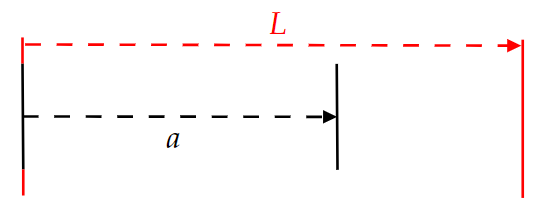
\includegraphics[width=0.5\linewidth]{img/1.png}
			\caption{The two nested one-dimensional boxes.}
		\end{figure}
		
		\noindent
		But if this energy somehow depends on the problem's characteristic scale, then the derivative of the Casimir energy with respect to that scale can have physical significance. Here we obtain the Casimir force for a simple one-dimensional setup.
	\end{problem}
	\begin{enumerate}
		\item
		\begin{problem}{\points{-}}
			\textbf{The setup:}
			
			\noindent
			Consider a one-dimensional box of length $a$, inside another box of length $L$, where $a<L$. The outer box is required to bypass some conceptual issues, and in the end, we take $L\xrightarrow{} \infty$ limit.
			
			\noindent
			Upon quantization, the discrete frequencies are $\omega_n = \frac{\pi}{a}n$ and $n\in \mathbb{N}$. Casimir energy is the sum of the energies of all the quantum states. Note that you have to sum energies associated with two boxes due to the presence of two boxes. One is for the original box of length $a$; the other one is for the remaining space, which has length $L-a$, since we've accounted for the D.O.Fs between length $[0,a]$.
			
			\noindent
			Write $E_{tot}(a)$, show that Casimir force, $F_{Casimir} = -\frac{dE_{tot}}{da}$ diverges.
		\end{problem}
		\item
		\begin{problem}{\points{-}}
		\textbf{Regularization of force via hard cut-off}
		
	This divergence arises partly because of our ignorance of super high-frequency modes. Walls are made of atoms, and super high-frequency modes will penetrate the small gap between the atoms; thereby it's not viable to sum over all energy states. Whether what modes will penetrate the wall is not our interest because it involves providing a theory for the wall's atoms. The crucial point is that we have to do the summation in part (a) up to modes that penetrate the wall.
	
	\noindent
	We employ a high-frequency cut-off $\Lambda$, $\omega <\pi\Lambda$. Then the allowable modes will have $n< n_{max} = [\Lambda a]$.\footnote{$[X]$ denotes the greatest integer less than or equal to $X$.} Now repeat the calculation in part (a), but instead up to $n=n_{max}$. Use $x = \Lambda a - [\Lambda a]$ to rewrite your expression in terms of $x$ and $\Lambda a$. (Suppose $[\Lambda a]$ is not an integer.) 
		\end{problem}
	\item
	\begin{problem}{\points{-}}
		\textbf{Averaging $x$ variable:}
		
		\noindent
		There still remains $x$, but it's finite and lies in interval $[0,1)$. We can eliminate this variable by averaging it. Do this averaging.
	\end{problem}

	\item
\begin{problem}{\points{-}}
	\textbf{The Casimir energy in the hard cut-off scheme:}
	
	\noindent
	Finally, take derivative with respect to $a$. And after derivation, you can take the $L\xrightarrow{} \infty$ without any concern.  What's the value of the Casimir force?
\end{problem}
\end{enumerate}

\newpage
	\section*{Problem 2: Regularization Schemes}

\begin{problem}
	As its name suggests, the model provided in the previous problem cuts off the UV modes hardly. Its form is $\theta(\pi \Lambda - \omega)$. We can forget the model and recruit other regularization schemes to find Casimir force. 
	
	\noindent
	Notice that we can use these schemes in calculating the determinant of operators, as you've seen in the class and gained familiarity in applying them. Here, we want you to reproduce the result of problem 1 in different schemes.
	

	
\end{problem}
\begin{enumerate}
	\item
	\begin{problem}{\points{-}}
		\textbf{Gaussian regularization:}
		
		\noindent
		Use Gaussian Kernel to evaluate the zero-point energy and Casimir force.
		\[
		E(r) = \frac12 \sum_n \omega_n e^{-(\frac{\omega_n}{\pi\Lambda})^2}
		\]
	\end{problem}
	\item
	\begin{problem}{\points{-}}
		\textbf{Zeta function regularization:}
		\noindent
		Use Zeta function Kernel to evaluate the zero-point energy and Casimir force.
		\[
		E(r) = \frac12 \sum_n \omega_n (\frac{\omega_n}{\mu})^{-s}
		\]
	\end{problem}

\end{enumerate}

	\textbf{Aside:} One can prove that the results are regulator-independent as long as regulators sastisfy certain criteria, namely:
	\[
	\lim_{x \to \infty } xf^j(x) =0, \;\;\;\;\;\;\;\;\;\;\;\;\;\;\; f(0) =1
	\]
	We can discuss them in the class if you'd like to.
\newpage

\section*{Problem 3: Point Particle Quantization by three different methods: Path Integral Labor - Faddeev Popov - BRST}
\begin{problem}
	As you know, the  relativistic free-particle action
	\[
	S_{0} = -m \int d\tau (-\eta_{\mu\nu}\dot{X}^\mu\dot{X}^\nu)^{-\frac12} 
	\] 
	suffers several ailments. So, we define another action involving einbein.
	\[
	S = \frac{1}{2}\int d\tau (e^{-1}(\tau) \dot{x}.\dot{x} - e(\tau) m^2)
	\]
	This formulation comes from putting a metric on the world line, a one-dimensional metric, with $g_{\tau\tau} = e^2(\tau)$. We can call it one-dimensional Polyakov action.
	
	\noindent
	In this problem, we approach its quantization with three methods. All of which are the same in their nature. To be more specific, the Faddeev-Popov method accounts for the gauge group volume by inserting a functional "1:, which is a functional representation of the Dirac delta. BRST tries to address this issue by introducing new fields to the problem.
	
	\noindent
Note that the problem may be challenging to solve. I, myself, even struggle with some parts of it! Please don't worry and proceed as much as you can.
\end{problem}	

	\begin{enumerate}
	\item
	\begin{problem}{\points{-}}
		\textbf{Warm-up:} 
		
		\noindent
		This action is reparametrization invariant, as suggested in your notes. Work out $\delta X^\mu$ and $\delta e$ under infinitesimal transformation $\tau \xrightarrow{} \tau + \xi(\tau)$.
		
		\noindent
		Then find the Equation of Motion (E.O.M) of $e(\tau)$. Find E.O.M of $x$ by varying action with respect to it. Show that by replacing back $e$ into E.O.M of $x^\mu$, you end up with the same E.O.M derived from the old action $S_0$.[Which is $\partial_\tau (\frac{m\dot{x}_\mu}{\sqrt{-\dot{X}^2}})=0$].
		
		\noindent This means that reparametrization serves as a gauge transformation for the action $S$, while it was hidden in $S_0$.
		
		
	\end{problem}
	\item
	\begin{problem}{\points{-}}
		\textbf{Path integral method - direct computation:}
		
		We evaluate the path integral by discretization. Notice that it's similar to the exercises that were solved beforehand. Except that you have to manage to integrate over gauge D.O.Fs properly!
		
		\noindent
		 Let's just focus on the propagator. Once we tackle the problem, it's not hard to generalize the problem.
		 
		 \[
		 \mathcal{N} \int_{x(0) = x}^{x(1) = x^{\prime}} \mathcal{D}e \mathcal{D}x^\mu e^{-\frac12 \int_0^1 (\frac1{e}\dot{x}^2 - em^2) d\tau}
		 \]
		 
		\noindent
		\begin{enumerate}
			\item 
			As you saw in (a), $\delta e = \partial_\tau (\xi e)$. To fix the gauge to a constant value, we choose $L = \int_0^1 \sqrt{g^{\tau\tau}}d\tau = \int_0^1 e(\tau) d\tau$. Argue why it must be fixed like this. By which I mean it should be equal to the length of the path and not any other constant.			
			\item  To proceed further, the integration over $e$, which is integration over metric parameters, has been vastly studied during World War II.\footnote{Even in the front of the war!} These parameters are called Teichmuller parameters. Fortunately, in one-dimensional metrics, it's easy to classify all the metrics and define an integration measure on the space of all metrics.
			
			\noindent
			The $e$-integration involves both scaling(constant modes) and reparametrization modes. We've removed the reparametrization invariance by the choice of the gauge ($L$), and there just remains to integrate over the scaling modes. This is realized via
			\begin{equation}
				\mathcal{N}\int_{0}^{\infty} dL \int_{x(0) = x}^{x(1) = x^{\prime}} \mathcal{D}e \mathcal{D}x^\mu e^{-\frac12 \int_0^1 (\frac1{L}\dot{x}^2 - Lm^2) d\tau}
				\label{pi}
			\end{equation}
			
			\noindent
			Up to now, I just motivated the above formula, now do the following tasks:
		
				\item Exapnd around classical path, and by working out $||\delta x^\mu||$(as done in your notes), conclude that measure would be $\mathcal{D}x^\mu = \prod \sqrt{L} d\delta x^\mu(\tau)$.
				\item Discretize and evaluate the path integral.(You've to end up to something proportional to $\det(-\frac{\partial^2_\tau}{L^2})^{-2}$).
				\item By spectral decomposition, we find that $\det(-\frac{\partial^2_\tau}{L^2}) = \prod_{n=1}^{\infty} \frac{n^2}{L^2}$. In this part, just regularize this infinite product via Zeta function regulator.
			\item \textbf{Optional!} Plug back into path integral \eqref{pi} and do a fourier transformation to find the usual Feynman propagator.
		\end{enumerate}
	\end{problem}

\begin{problem}{\points{-}}
	\textbf{Faddeev-Popov procedure} 
	
	\noindent
	As mentioned, it involves adding a functional "1". This functional "1", magically takes gauge group volume into consideration, as you will see in this part.
	
	\begin{enumerate}
		\item Define $1 = \Delta(e) \int \mathcal{D}\xi \delta(e-L[\xi])$, where $L[\xi]$ is value of the constant einbein after gauge transformation. Now just plug this into path integral \eqref{pi}.
		\item Do the integral over $e$, now that there is a functional Dirac delta function, you can do this very very easy!
		\item Since the integrand is gauge invariant, do a gauge transformation to drop $\xi-$dependence of your exponential part and $L[\xi]$. Then factor out the path integral on $\mathcal{D}\xi$, which produces the volume of gauge group, and accounts for gauge D.O.Fs. (This part is rather formal, no need to write a solution, just explain the ellimination of $\xi$.)
		\item Now try to solve for $\Delta(L)$ from the part (i). Use integral representation of Dirac delta function. At the end you should plug this into the result of part (iii), and end up with propagator's form.
	\end{enumerate}
	
	
\end{problem}

\begin{problem}{\points{-}}
	\textbf{BRST quantization} 
	
	\noindent
	We're not going to delve into this completely, but it's going to be a very long introduction to BRST.
	
	\noindent
	 The BRST approach compensates for the gauge D.O.Fs in the Lagrangian by another method, adding new auxiliary fields with (anti-)commuting Grassmann fields. This approach is very powerful to fix gauge in ANY gauge thoery to ANY function. It involves promoting symmetry of the Lagrangian to a larger symmetry called BRST symmetry. This symmetry is crucial to show the independence of  physical results from different gauges and construct consistent Hilbert space of the theory.
	 
	 \noindent
	 Define BRST transformations by:
	 \begin{equation}
	 	\begin{aligned}
	 		\delta_{BRST} (x^\mu) &= \Lambda c e^{-1}\dot{x}^\mu \\
	 		\delta_{BRST} (e) & = \Lambda \dot{c} \\
	 		\delta_{BRST} (c) & = 0 \\
	 		\delta_{BRST} (b) & = i\Lambda \pi \\
	 		\delta_{BRST} (\pi) & = 0 \\
	 	\end{aligned}
	 \end{equation}
	Where $c(\tau)$ is an auxiliary ghost, real Grassmann field. $\Lambda$ is pure imaginary Grassmann number (independent of $\tau$) called BRST parameter. $b(\tau)$ is anti-ghost, Grassmann field, and $\pi(\tau)$ is a usual commuting field.
	
	\noindent
	We also add gauge fixing term to action. Consider you want to fix gauge freedom (e) to an arbitrary function $f(x,e,\pi)$, define $\Psi = \int_0^1 d\tau\; b(\tau) f(x,e,\pi)$. Then add $S_{\textbf{fix}}[x,e,c,b,\pi] = \frac{\delta}{\delta \Lambda} \Psi$ to your action, where $\frac{\delta}{\delta \Lambda} \Psi$ means BRST transformation of $\Psi$ with the parameter $\Lambda$ removed from the left.
	
	\noindent
	Up to now, your action is $S_q \equiv S[x,e] +S_{\textbf{fix}}[x,e,c,b,\pi]$. The path integral would be
	\[
	Z = \int \mathcal{D}x\mathcal{D}e\mathcal{D}c\mathcal{D}b\mathcal{D}\pi e^{-S_q}
	\]
	explicitly, well-defined for any choice of $f(x,e,\pi)$. We call $S_q$ gauge-fixed BRST-invariant action.
	\begin{enumerate}
		\item Show that this is a symmetry of the action $S$. ($\delta_{BRST}(S) = 0$)
		\item Fix the freedom with the choice $e=L$ or $f(x,e,c,b,\pi) = L-e$, compute $S_{\textbf{fix}}$ from the definition of $\Psi$.
		\item Write out the path integral expression, you'll see that integral over $\pi$ results a functional Dirac delta function on e, so that you can evaluate $e$-integration. This is pretty similar to Faddeev-Popov procedure.
		
		\noindent
		Finally reach at $Z = \int\mathcal{D}x\mathcal{D}c\mathcal{D}b \; e^{-\int_0^1 dx \big(\frac{\dot{x}^2}{2L} + \frac{L}{2} m^2 +b\dot{c}\big)}$. Where the integration on $b$,$c$ ghosts will produce the same $\det(\partial_\tau)$ on the Faddeev-Popov procedure.
		
		\noindent
		This is the end of the story. You can proceed by this action to do perturbative calculation, including ghost vertices in your Feynman diagrams. All the  well-known QFT identites and observations satisfied in any perturbative order.
	\end{enumerate}
	
	
\end{problem}



\end{enumerate}

\newpage
\section*{Problem 4: Free Fermionic Path integral and miscellaneous derivations}

\begin{problem}
	We've looked at Fermionic path integrals before. Here, we complete our discussion.
	
	\noindent
	Also, There were some minor derivation steps that I mentioned during the recorded assistant classes, and we investigate some of them here.
	
	
	
\end{problem}
\begin{enumerate}
	\item
	\begin{problem}{}
		\textbf{Fermionic Path Integral:}
		\begin{enumerate}
			\item
			Generalize the Grassmann integral you've encountered in problem set 2, prove the following relation:
			\[
			\int d\bar{\theta}_1 \dots d\bar{\theta}_n d\theta_1 \dots d\theta_n 
			e^{-\sum_{ij}\bar{\theta}_i A_{ij}\theta_j + \sum_i \bar{\eta}_i\theta_i + \sum_i \bar{\theta}_i \eta_i} = \det(A) e^{\sum{ij}\bar{\eta}_i A^{-1}_{ij}\eta_j}
			\]
			\item Define $(i\gamma^\mu\partial_\mu -m)^{-1}$ by $(i\gamma^\mu\partial_\mu -m)\Pi(x-y) = -i\delta(x-y)$, then do a Fourier transformation and find the usual propagator.
			\item Now evaluate $Z[\bar{\eta},\eta] = \int \mathcal{D}\bar{\Psi}\mathcal{D}\Psi e^{i\int d^4x \bar{\Psi}(x)(i\gamma^\mu\partial_\mu -m)\Psi + \bar{\eta}\Psi + \bar{\Psi}\eta}$.
			\item Compute the following four-point function, with the definition of the generating functional.
			\[
			\bra{0}T\{\Psi(x_1)\bar{\Psi}(x_2)\Psi(x_3)\bar{\Psi}(x_4)\}\ket{0}
			\]
		\end{enumerate}
		
	\end{problem}
	\item
	\begin{problem}{\points{-}}
		\textbf{Miscellaneous:}
		\begin{enumerate}
			\item As we saw in the assistant class, an innocent shift in path integral measure will benefit us overwhelmingly! Prove the Schwinger-Dyson equation (pursue the same line followed in the class.)
			\[
			-i\Box_x \frac{\partial Z[J]}{\partial J(x)} = \Bigl\{\mathscr{L}_{int}^{\prime}[-i\frac{\partial}{\partial J(x)}]+ J(x)\Bigr\} Z[J]
			\]
			\item In proving gauge invariance, I showed that adding the $-\frac{1}{2\xi}(\partial_\mu A^\mu)^2$ doesn't affect correlation functions of a gauge-invariant operator. What about $-\frac{1}{2\xi}(\partial_\mu A^\mu)^4$ or $\xi A^\mu A_\mu$?
		\end{enumerate}
	\end{problem}
	
\end{enumerate}









\end{document}